\section{Single physical user} \label{sec:single-user}

Considering a single user in the conference room, the SINR of that user will be very high compared to a scenario with more than one physically present user. This has to do with having no intra-cell interference because no other transmissions are performed by the serving \acs{BS}. Since intra-cell interference is the only interference term we may have in a single panel transmission, the total interference is zero and the SINR degenerates in an SNR, reaching values well above the 30 dB mark.

% Section of the BLER CURVES
From the analysis of the BLER curves (Figure \ref{fig:blercurves} in section ???), when operating with such high SINRs the probability of occurring block errors is practically zero. Hence the bit rate is either constrained by the available bits in the buffer or by the maximum possible bit rate a user can have, and we must identify which situation it is. Figure \ref{fig:su_bitrate} shows the instantaneous bit rate in each TTI and the average bit rate of the past 800 TTIs, or 200 ms, the duration of a \ac{GoP}.

We can see the instantaneous bit rate oscillates between 190 and 145 Mbps, approximately. Therefore what is limiting the bit rate is the lack of bits in the buffer, otherwise there would be no realised bit rate oscillations since the maximum achievable bit rate is constant for a constant MCS, which is the case in scenarios with extremely-high \acsp{SINR}.

% VERY IMPORTANT NOTE:
% - should we call it bit rate or throughput? -> it is a bit rate, we are using no overheads, considering only DL slots and the ideal case where all slots are self-contained and have no latency constraints.
% - as a way of establishing a baseline for what is physically possible.

\imagecapcontrol{Results/su_bitrate.pdf}{ffddf}{fig:su_bitrate}{.7}{-3mm}


Additionally, performing the computation for the highest achievable bit rate under ideal conditions, i.e. no block errors, using the highest \acs{MCS}, and all 50 \acsp{PRB}: the system should support 250 Mbit/s. We must guarantee there are enough packets in the buffer in order not to limit the possible experienced bit rate. So, we set $\overline{R}_{DL}$ from 80 Mbps to 500 Mbps exclusively to plot the maximum achievable bit rate in Figure \ref{fig:su_bitrate_full}. 

\imagecapcontrol{Results/su_bitrate_full.pdf}{bit rate 'full buffer'}{fig:su_bitrate_full}{.73}{-3mm}

Contrary fo Figure \ref{fig:su_bitrate}, there is no instantaneous bit rate oscillations in Figure \ref{fig:su_bitrate_full} because the quantity of bits in the buffer always exceeds the bits to be sent that TTI. The zero-bit rate TTIs are due to an empty buffer - packets get discarded if the scheduler realises they are going to exceed the latency constraints and excess packets come from setting the average arrival rate so high.

Thus we may conclude that maximum average achievable bit rate for a user under the described conditions is roughly 175 Mbps, reaching 250 Mbps in instantaneous bit rate. And observe that the latency plays an important role. The higher the latency, the closer to the maximum instantaneous bit rate the average bit rate gets. 

From the two graphs above we derive two important conclusions: from Figure \ref{fig:su_bitrate} we conclude the deployment and network configurations support an average bit rate of 80 Mbps in the \ac{DL} for one user; and from Figure \ref{fig:su_bitrate_full} we set the threshold for what is the maximum bit rate a user can achieve. To further expand this quantity, other strategies need to be used, like using an higher MCS or multi-layer transmission.

Finally, is important to note that a conference use-case with only one user is a scenarios where the resource distribution is trivial and very high bit rates are expected. In the next section we consider a more demanding case of having multiple users to serve simultaneously.



\section{Multiple physical users} \label{sec:multi-user}

Let us now consider a more demanding scenario with four physical users, each with a downlink average bit rate of 80 Mbps. Analogously to the first figure in the previous section, Figure \ref{fig:mu_bitrates} represents the instantaneous bit rate as well as the average bit rate of the last 800 TTIs, for each of the present users. Here we see the influence of a more chaotic, and realistic, channel.

\imagecapcontrol{Results/mu_bitrate.pdf}{bit rate, instantaneous and averaged over the last 800 TTIs}{fig:mu_bitrates}{.73}{-3mm}

% here the case for oscillations is block errors and channel variation
In Figure \ref{fig:mu_bitrates}, the cause for bit rate oscillations may not only be the same as in the previous section, i.e. variability of packet arrival rate on a TTI-basis, but also the variability of channel conditions. As such, this section is dedicated to carefully dissect what is happening.

A good indicator of the channel quality variability is the SINR each user experiences. Figure \ref{fig:mu_sinr} shows such \acsp{SINR}, the estimated from channel measurements and the realised from the actual transmission. The variable experienced received signal power and interference power are represented in Figure \ref{fig:mu_pow}.

\imagecapcontrol{Results/mu_sinr.pdf}{SINR, estimated before transmission and experienced during transmission}{fig:mu_sinr}{.73}{-3mm}

\imagecapcontrol{Results/mu_pow_vs_inter.pdf}{Received Signal and Interference Powers}{fig:mu_pow}{.73}{-1mm}

Figure \ref{fig:mu_pow} shows abnormally high received signal powers. Taking into account the \acs{BS} transmit power is 100 mW, we can see that some \acsp{UE} are receiving more than that, which is certainly wrong. However, it seems to be a problem merely with the scale because all of them are consistent and lead to realistic \acsp{SINR}. We hypothesise the scale should be in dBm instead of dBW, but further verifications need to be done.

And, the justification for the step-like experienced SINRs has to do with only updating the variable that holds the SINR when there are transmissions. Thus when the buffer is empty the variable is not updated and stays constant. 

Nonetheless, the previous two figures are consistent. Furthermore, we see the channel varies significantly and in unpredictable ways for each user. With such accentuated channel variability, the highest MCS that is predicted to result in less block errors than our BLER target also changes. This fact alone justifies variable bit rates.

Figure \ref{fig:mu_mcs} shows the \ac{MCS} index used for the transmissions to each \acs{UE}. Assuming the same degree of block errors, the higher the average MCS index, the more likely a user is to get an higher bit rate. We see this relation when comparing the achieved bit rates in Figure \ref{fig:mu_bitrates} and the MCS used for each transmission, below.


\imagecapcontrol{Results/mu_cqi.pdf}{MCS index ....}{fig:mu_mcs}{.73}{-3mm}

As expected, sufficient channel variability causes changes in the experienced bit rate. Furthermore, channel variability may lead to block errors, since predicting the future state of the channel constitutes no trivial task and even the slightest drifts between SINR estimation and realisation can using the incorrect MCS and result errors in the transmitted transport blocks.

Figure \ref{fig:mu_bler} shows the average BLER across time. And one clearly testifies that all users experience blocks with errors.

This Figure agrees with what we have seen so far. For instance, in case of \ac{UE} 2, we can identify that right after the 2500 TTI mark the BLER monotonically decreases. This happens because the experienced SINR has passed the point of where BLER probability is noticeable, and every block has practically zero chance of having errors. By analysing the \acs{MCS} curves (Figure \ref{fig:blercurves}), we see that \acsp{SINR} above 26 dB, approximately, results in virtually no block errors, therefore driving the average BLER down. And UE 2 passes this 26 dB threshold around the 2500 TTI mark too, like we observe from Figure \ref{fig:mu_sinr}.

\imagecapcontrol{Results/mu_running_bler.pdf}{All time BLER average in a multi-user scenario.}{fig:mu_bler}{.73}{-3mm}


To cope with the channel variability we use a link adaptation method that adjusts the MCS according to the block errors detected. Figure \ref{fig:mu_olla} shows the instantaneous \acs{BLER} for UE 2 and how the OLLA parameter varies accordingly. On close inspection, $\Delta_{OLLA}$ rises when there are transmissions without errors and decreases when there are transmissions where blocks had errors. This behaviour leads to choosing a lower MCS when there are errors and slowly opting for an higher MCS when the channel is better than expected. Only when there are transmissions (zones marked in grey) there are blocks with or without errors. Naturally therefore, the \acs{OLLA} parameter is not updated outside of the such zones.

\begin{center}

    \hfill 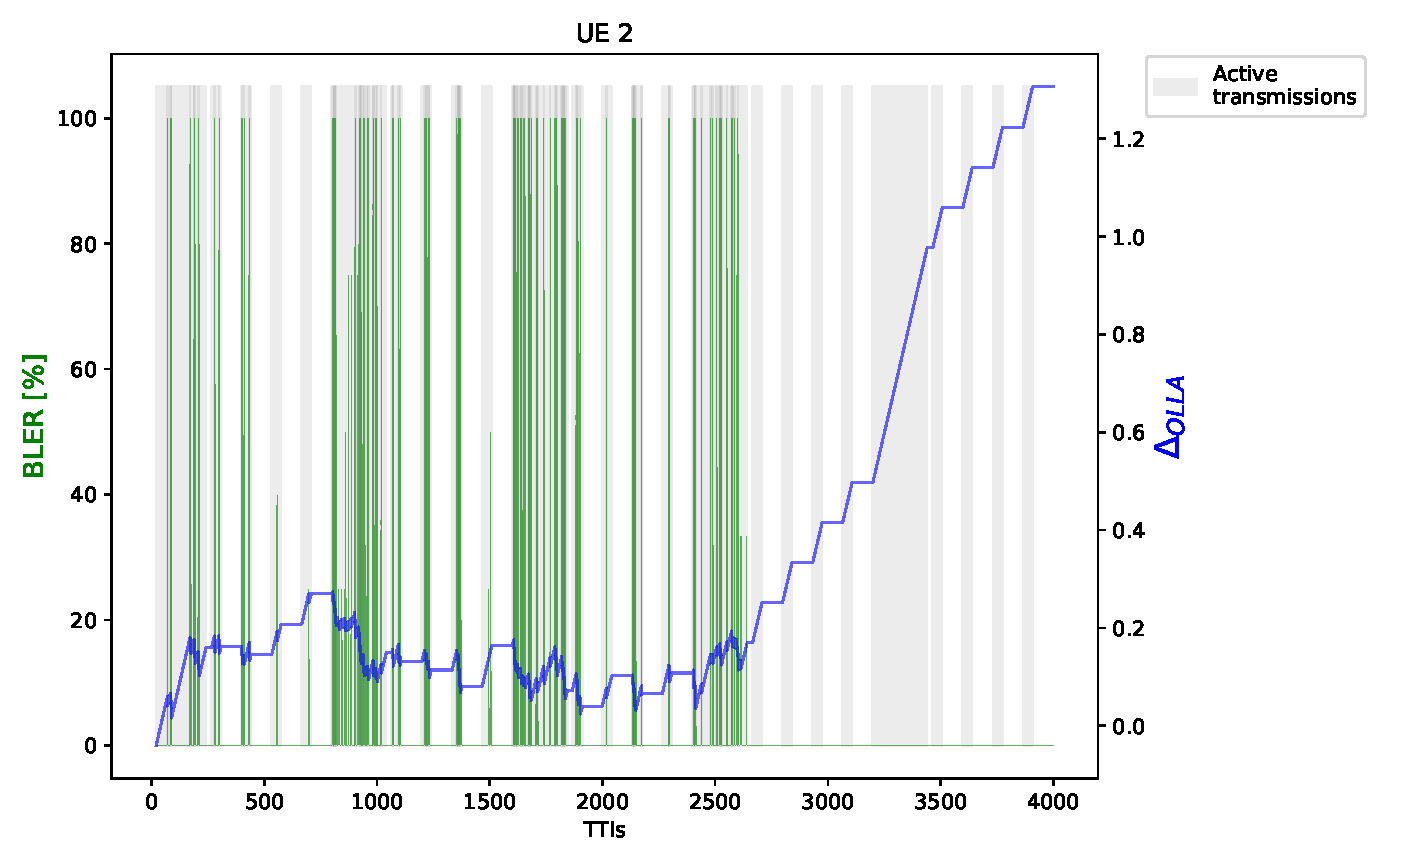
\includegraphics[scale = .6]{Results/mu_olla3.pdf}
    \captionsetup{type=figure} 
    \vspace{-3mm}   
    \caption{Link adaptation parameter variation with the instantaneous \acs{BLER}. Grey zones mark when the UE has active transmissions.}			
    \label{fig:mu_olla}
    
\end{center}

The use of this link adaptation scheme should make the BLER converge to the BLER target of 10\%. It still is uncertain why that does not happen and requires further investigation.

Finally, much like the previous section, we can derive some conclusions regarding how well the deployment and configurations cope with the requirements. However, it should not be taken as a final statement since some modelling simplifications listed in the beginning of this chapter were considered, some results are yet to be understood, and perhaps require rectifications, and this analysis lacks statistical significance: we cannot derive such conclusions by looking at one second of one use-case. But we can conclude something about that one second despite all limiting factors.

Nevertheless, to conclude something relevant we cannot resort exclusively to bit rate plots since those say nothing about performance with respect to latencies. From the application perspective, we want to answer questions such as: ``what is maximum application throughput that achieves less than X \% packet error rate?''

That is a difficult question, but we can take another sizeable step towards answering it, and also a step towards improving whatever that answer may be. That step consists in understanding in what circumstances the high packet loss occurs. 

Figure \ref{fig:mu_lat} shows the horizontal axis as frame indices instead of TTIs - they have a direct mapping: five GoP (each of duration 200 ms) are sent in one second, or 4000 TTIs. Furthermore, the I-frames have indices \{0, 6, 12, 18, 24\} and are marked in red. In the figure we can see the correlation between the average latency of packets belonging to the same frame and the packet drop rate for that frame. More importantly, we see as a general rule that both rise right after an I-frame.

\imagecapcontrol{Results/lat_drop_rate.pdf}{Packet latencies and drop-rates ...}{fig:mu_lat}{.65}{-3mm}

We can notice that when packets are dropped, they are not dropped equally amongst all users - the percentage of dropped packets changes and the frame they belong to changes as well. If packets are dropped after the I frame, it means the link had enough quality to cope with the I frame, but having a P frame following with no pause led to the delay of some packets past the latency requirement. This is the case when the drop rate peak comes after the I-frame, which is the most common case. And the lower the drop rate peak is, the closer the user was to handling all packets within the required time. 

Another more extreme case is when the peak of the packet drop rate occurs during the I-frame transmission (e.g. the third I-frame of UE 0). This means that not all packets from that I-frame were sent within the latency budget.

Comparing Figures \ref{fig:mu_sinr} and \ref{fig:mu_lat} for UE 0 we see how the worst case in terms of packet average latency and drop rate clearly aligns with the worst experienced SINR across all users, at the 1500 TTI mark.

